\documentclass[11pt]{article}
\usepackage[a4paper,margin=21mm]{geometry}
\usepackage{fontspec}
\setmainfont{Latin Modern Roman}
\newfontfamily\CJKfont{Noto Serif CJK SC}
\XeTeXlinebreaklocale "zh"
\XeTeXlinebreakskip=0pt plus 1pt
\usepackage{amsmath,amssymb,amsthm,amscd,graphicx,color}
\usepackage{xurl}
\usepackage[unicode,hidelinks]{hyperref}
\allowdisplaybreaks
\setlength\emergencystretch{3em}
\numberwithin{equation}{section}
\usepackage{mathtools,mathrsfs,enumerate,tikz,tikz-cd,bm}
% Independently written finite AMS notation bindings for1223 only.
% Unknown mypackage_WRT/mycommand_WRT implementations are not imported.
\newcommand{\veps}{\varepsilon}
\newcommand{\Z}{\mathbb{Z}}
\newcommand{\Q}{\mathbb{Q}}
\newcommand{\R}{\mathbb{R}}
\newcommand{\bbC}{\mathbb{C}}
\newcommand{\bbH}{\mathbb{H}}
\newcommand{\calL}{\mathcal{L}}
\DeclareMathOperator{\SL}{SL}
\DeclareMathOperator{\SU}{SU}
\renewcommand{\theenumi}{(\roman{enumi})}
\renewcommand{\labelenumi}{\theenumi}
\renewcommand{\theenumii}{(\alph{enumii})}
\renewcommand{\labelenumii}{\theenumii}
\makeatletter\renewcommand{\p@enumii}{}\makeatother
\newif\ifsigmaFiniteAllowed
\expandafter\def\csname sigmaApprovedpmat0\endcsname{w_1 & 1 & 1 & 1 & 0 & 0 \\
	1 & w_2 & 0 & 0 & 1 & 1 \\
	1 & 0 & w_3 & 0 & 0 & 0 \\
	1 & 0 & 0 & w_4 & 0 & 0 \\
	0 & 1 & 0 & 0 & w_5 & 0 \\
	0 & 1 & 0 & 0 & 0 & w_6 }
\expandafter\def\csname sigmaApprovedpmat1\endcsname{Ma & MNb \\ MNb & Nc}
\expandafter\def\csname sigmaApprovedpmat2\endcsname{c & -Nb \\ -Mb & a}
\expandafter\def\csname sigmaApprovedpmat3\endcsname{M & 0 \\ 0 & N}
\expandafter\def\csname sigmaApprovedpmat4\endcsname{(1 - MM^*) \alpha \\ (1 - NN^*) \beta}
\newcommand{\pmat}[1]{\begingroup\def\sigmaActualArgument{#1}\sigmaFiniteAllowedfalse
\expandafter\ifx\csname sigmaApprovedpmat0\endcsname\sigmaActualArgument\sigmaFiniteAllowedtrue\fi
\expandafter\ifx\csname sigmaApprovedpmat1\endcsname\sigmaActualArgument\sigmaFiniteAllowedtrue\fi
\expandafter\ifx\csname sigmaApprovedpmat2\endcsname\sigmaActualArgument\sigmaFiniteAllowedtrue\fi
\expandafter\ifx\csname sigmaApprovedpmat3\endcsname\sigmaActualArgument\sigmaFiniteAllowedtrue\fi
\expandafter\ifx\csname sigmaApprovedpmat4\endcsname\sigmaActualArgument\sigmaFiniteAllowedtrue\fi
\ifsigmaFiniteAllowed \begin{pmatrix}#1\end{pmatrix}\else\PackageError{sigma1223}{Unobserved pmat argument}{Only exact source inventory arguments are supported}\fi\endgroup}
\expandafter\def\csname sigmaApprovedsprod0\endcsname{\cdot, \cdot}
\expandafter\def\csname sigmaApprovedsprod1\endcsname{x, h(y)}
\expandafter\def\csname sigmaApprovedsprod2\endcsname{x, y}
\expandafter\def\csname sigmaApprovedsprod3\endcsname{y, h(y)}
\expandafter\def\csname sigmaApprovedsprod4\endcsname{x, h(x)}
\expandafter\def\csname sigmaApprovedsprod5\endcsname{x, z}
\expandafter\def\csname sigmaApprovedsprod6\endcsname{y + z, h^{-1}(y + z)}
\newcommand{\sprod}[1]{\begingroup\def\sigmaActualArgument{#1}\sigmaFiniteAllowedfalse
\expandafter\ifx\csname sigmaApprovedsprod0\endcsname\sigmaActualArgument\sigmaFiniteAllowedtrue\fi
\expandafter\ifx\csname sigmaApprovedsprod1\endcsname\sigmaActualArgument\sigmaFiniteAllowedtrue\fi
\expandafter\ifx\csname sigmaApprovedsprod2\endcsname\sigmaActualArgument\sigmaFiniteAllowedtrue\fi
\expandafter\ifx\csname sigmaApprovedsprod3\endcsname\sigmaActualArgument\sigmaFiniteAllowedtrue\fi
\expandafter\ifx\csname sigmaApprovedsprod4\endcsname\sigmaActualArgument\sigmaFiniteAllowedtrue\fi
\expandafter\ifx\csname sigmaApprovedsprod5\endcsname\sigmaActualArgument\sigmaFiniteAllowedtrue\fi
\expandafter\ifx\csname sigmaApprovedsprod6\endcsname\sigmaActualArgument\sigmaFiniteAllowedtrue\fi
\ifsigmaFiniteAllowed \left\langle#1\right\rangle\else\PackageError{sigma1223}{Unobserved sprod argument}{Only exact source inventory arguments are supported}\fi\endgroup}
\expandafter\def\csname sigmaApprovedabs0\endcsname{z_v}
\expandafter\def\csname sigmaApprovedabs1\endcsname{q}
\expandafter\def\csname sigmaApprovedabs2\endcsname{z_{v}}
\expandafter\def\csname sigmaApprovedabs3\endcsname{L'/L}
\expandafter\def\csname sigmaApprovedabs4\endcsname{\det h}
\expandafter\def\csname sigmaApprovedabs5\endcsname{w_{v}}
\newcommand{\abs}[1]{\begingroup\def\sigmaActualArgument{#1}\sigmaFiniteAllowedfalse
\expandafter\ifx\csname sigmaApprovedabs0\endcsname\sigmaActualArgument\sigmaFiniteAllowedtrue\fi
\expandafter\ifx\csname sigmaApprovedabs1\endcsname\sigmaActualArgument\sigmaFiniteAllowedtrue\fi
\expandafter\ifx\csname sigmaApprovedabs2\endcsname\sigmaActualArgument\sigmaFiniteAllowedtrue\fi
\expandafter\ifx\csname sigmaApprovedabs3\endcsname\sigmaActualArgument\sigmaFiniteAllowedtrue\fi
\expandafter\ifx\csname sigmaApprovedabs4\endcsname\sigmaActualArgument\sigmaFiniteAllowedtrue\fi
\expandafter\ifx\csname sigmaApprovedabs5\endcsname\sigmaActualArgument\sigmaFiniteAllowedtrue\fi
\ifsigmaFiniteAllowed \left\lvert#1\right\rvert\else\PackageError{sigma1223}{Unobserved abs argument}{Only exact source inventory arguments are supported}\fi\endgroup}

\numberwithin{equation}{section}

\newtheorem{Theorem}{Theorem}[section]
\newtheorem{cor}[Theorem]{Corollary}
\newtheorem{lem}[Theorem]{Lemma}
\newtheorem{prop}[Theorem]{Proposition}
 { \theoremstyle{definition}
\newtheorem{dfn}[Theorem]{Definition}
\newtheorem{Note}[Theorem]{Note}
\newtheorem{ex}[Theorem]{Example}
\newtheorem{rem}[Theorem]{Remark}
\newtheorem{assump}[Theorem]{Assumption}
}

\usetikzlibrary{knots}
\usetikzlibrary{positioning}

\newcommand{\trans}[1]{#1^\top}

\begin{document}
\begin{center}\Large WRT invariants as radial homological-block limits for negative-definite unimodular six-vertex H-plumbings with leaf weights at most minus two\end{center}
\noindent\textbf{Stable ID:} 1223\quad\textbf{Author:} Akihito Mori; Yuya Murakami\par
\noindent\textbf{Work:} Witten-Reshetikhin-Turaev Invariants, Homological Blocks, and Quantum Modular Forms for Unimodular Plumbing H-Graphs\par
\noindent\textbf{Source:} \url{https://sigma-journal.com/2022/034/}\par
\noindent\textbf{Version:} Official SIGMA 18 (2022) article 034, DOI 10.3842/SIGMA.2022.034; journal PDF and native TeX acquired 2026-09-30, exact bytes pinned by SHA256\par
\noindent\textbf{Rights:} CC BY 4.0. Authors retain copyright. \url{https://creativecommons.org/licenses/by/4.0/}. Reuse and typesetting adaptation; original language and mathematical content preserved.\par
\noindent\textbf{Difficulty (prior selection preserved):} {\CJKfont H3: The proof resolves incomplete surgery Gauss sums by deriving weighted cancellations for the two-variable plumbing quadratic form. It matches a two-variable Euler-Maclaurin radial expansion to finite Bernoulli-weighted sums, then explicitly transforms the Kirby-color surgery expression through reciprocity. The new vanishing identities supply precisely the missing lattice terms, making the radial-limit formula rigorous beyond formal q-series or cited Seifert formulas.}\par
\medskip\noindent\textbf{Editorial boundary note (not author text):} Selected author obligation is exactly Theorem1.1 identity(1.2) for a negative-definite determinant-one six-vertex H plumbing with all negative weights, leaf weights w3–w6<=-2 and integer level k>=3. The full printed theorem is preserved, with standard principal-value homological block and S3-normalized WRT convention, full linking/surgery diagrams and all inputs. Complete current weighted Gauss cancellations, every local arithmetic proof, two-variable Euler-Maclaurin expansion/lattice-completion proof and full surgery/reciprocity/Bernoulli route are retained. Existing surgery, Gauss reciprocity, Euler-Maclaurin and homological-block representation formulas remain precisely stated author prerequisites. General auxiliary statements, Seifert/degenerate-normalization cases and later quantum modularity receive no separate counts; auxiliary gamma wording remains literal and is applied only on the nonzero plumbing-weight support. A bounded independently written standard AMS wrapper binds exactly the12 approved notation names and rejects unobserved pmatrix/paired-angle/absolute-value arguments against the exact6/8/7 inventory. Native body/list labels and every sign/index/order remain unchanged. Both unknown private styles and the original ZIP containing them are never executed or exported; exact licensed article TXT is the portable source binding. Unused unavailable extarrows import is omitted after zero retained-call inventory.\par
\medskip\hrule\medskip\noindent\textbf{Author text begins below.}\par
\setcounter{section}{0}
% Original source lines 59--59
\section{Introduction} \label{sec:intro}

\setcounter{section}{1}\setcounter{equation}{0}
% Original source lines 78--258
H-graphs shown in Figure \ref{fig:H-graph} are the simplest graphs which are not such graphs.
It is expected that H-graphs yield non-Siefert manifolds.
\begin{figure}[h]	\centering
		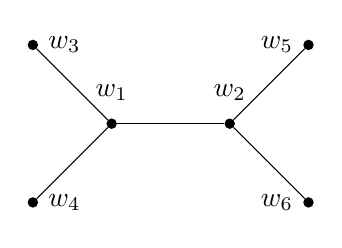
\begin{tikzpicture}
			\node[shape=circle,fill=black, scale = 0.4] (1) at (0,0) { };
			\node[shape=circle,fill=black, scale = 0.4] (2) at (1.5,0) { };
			\node[shape=circle,fill=black, scale = 0.4] (3) at (-1,-1) { };
			\node[shape=circle,fill=black, scale = 0.4] (4) at (-1,1) { };
			\node[shape=circle,fill=black, scale = 0.4] (5) at (2.5,1) { };
			\node[shape=circle,fill=black, scale = 0.4] (6) at (2.5,-1) { };
			
			\node[draw=none] (B1) at (0,0.4) {$ w_1 $};
			\node[draw=none] (B2) at (1.5, 0.4) {$ w_2 $};
			\node[draw=none] (B3) at (-0.6,1) {$ w_3 $};
			\node[draw=none] (B4) at (-0.6,-1) {$ w_4 $};
			\node[draw=none] (B5) at (2.1,1) {$ w_5 $};		
			\node[draw=none] (B6) at (2.1,-1) {$ w_6 $};	
			
			\path [-](1) edge node[left] {} (2);
			\path [-](1) edge node[left] {} (3);
			\path [-](1) edge node[left] {} (4);
			\path [-](2) edge node[left] {} (5);
			\path [-](2) edge node[left] {} (6);
		\end{tikzpicture}
		\caption{The H-graph $ \Gamma $.}\label{fig:H-graph}
	\end{figure}

In the case of H-graphs, Bringmann--Mahlburg--Milas~\cite{BMM} showed that radial limits of homological blocks coincide with sums of radial limits of multiple Eichler integrals.
Moreover, they proved that the radial limits of a homological block make up a quantum modular form of depth two and of weight one with the quantum set $ \mathbb{Q} $.

Meanwhile, for non-Seifert manifolds, it remains to be seen whether WRT invariants relate to homological blocks \cite[Conjecture~2.1]{GPPV} and have modularity.

In this paper, we study WRT invariants of H-graphs.
We will write them explicitly as weighted Gauss sums.
Moreover, we will prove that they relate to homological blocks and they yield quantum modular forms of depth two and of weight one with the quantum set $ \mathbb{Q} $.

Let us explain our setting.
Let $ \Gamma $ be the H-graph with vertices $ 1, \dots, 6 $ and weights $ w_v \in \Z_{<0} $ for each vertex $ v $ shown in Figure~\ref{fig:H-graph} such that its linking matrix
\begin{gather*}
W = \pmat{w_1 & 1 & 1 & 1 & 0 & 0 \\
	1 & w_2 & 0 & 0 & 1 & 1 \\
	1 & 0 & w_3 & 0 & 0 & 0 \\
	1 & 0 & 0 & w_4 & 0 & 0 \\
	0 & 1 & 0 & 0 & w_5 & 0 \\
	0 & 1 & 0 & 0 & 0 & w_6 }
\end{gather*}
is negative definite and its determinant is $ 1 $.


Then we obtain the link $ \calL(\Gamma) $ defined by $ \Gamma $ shown in Figure \ref{fig:surgery_diagram}.
Let $M_3(\Gamma)$ be the plumed 3-ma\-nifold obtained from $ S^3 $ through the surgery along the diagram $ \calL(\Gamma) $.
We obtain $H_1(M_{3}(\Gamma), \Z)\allowbreak \cong \Z^{6} / W\big(\Z^{6}\big)$ by use of the Mayer--Vietoris sequence.
Since $\det W = 1$, $M_{3}(\Gamma)$ is an integral homology sphere.
\begin{figure}[h]	\centering
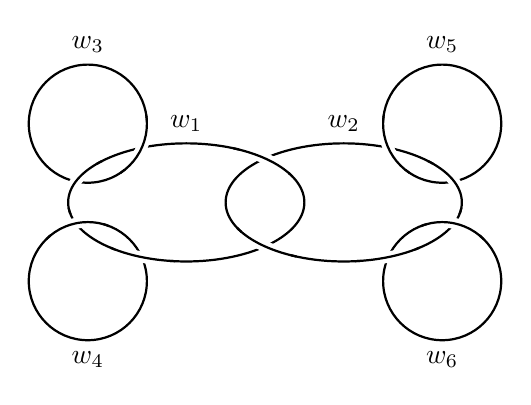
\begin{tikzpicture}[scale=0.5]
			\begin{knot}[
				clip width=5,
				flip crossing=2,
				flip crossing=4,
				flip crossing=6,
				flip crossing=7,
				flip crossing=9
				]
				\strand[thick] (0, 0) circle [x radius=3cm, y radius=1.5cm];
				\strand[thick] (0, 0) +(4cm, 0pt) circle [x radius=3cm, y radius=1.5cm];
				\strand[thick] (0, 0) +(-2.5cm, 2cm) circle [radius=1.5cm];
				\strand[thick] (0, 0) +(-2.5cm, -2cm) circle [radius=1.5cm];
				\strand[thick] (0, 0) +(6.5cm, 2cm) circle [radius=1.5cm];
				\strand[thick] (0, 0) +(6.5cm, -2cm) circle [radius=1.5cm];
				
				\node (1) at (0, 2) {$w_{1}$};
				\node (2) at (4, 2) {$w_{2}$};
				\node (3) at (-2.5, 4) {$w_{3}$};
				\node (4) at (-2.5, -4) {$w_{4}$};
				\node (5) at (6.5, 4) {$w_{5}$};
				\node (6) at (6.5, -4) {$w_{6}$};
			\end{knot}
		\end{tikzpicture}
\caption{The surgery diagram $ \calL(\Gamma) $ corresponding to $\Gamma$.}\label{fig:surgery_diagram}
\end{figure}

{\samepage
Such H-graphs yield Seifert manifolds if $ w_v = -1 $ for some $ 3 \le v \le 6 $.
Bringmann--Mahlburg--Milas~\cite[Theorem~1.2]{BMM} showed that there exist precisely $ 39 $ equivalence classes of such H-graphs with $ w_v \le -2 $ for each $ 3 \le v \le 6 $ up to graph isomorphism.

}

For a positive integer $k$, let $\tau_k$ be the WRT invariant normalised as $\tau_{k}\big(S^{3}\big) = 1$.
We study a~relation between the WRT invariant $\tau_{k}(M_{3}(\Gamma))$ and the homological block $\widehat{Z}_\Gamma (q)$.

For each complex number $ z $, we denote $ \bm{e}(z) := {\rm e}^{2\pi {\rm i} z} $.
For a point $ \tau \in \bbH $, let $ q := \bm{e}(\tau) $.
Gukov--Pei--Putrov--Vafa~\cite[formula~(3.145)]{GPPV} defined the homogical block $ \widehat{Z}(q) $ of the plumed graph.
In~our case, it can be written as
\begin{gather}
\widehat{Z}_\Gamma (q)		= \widehat{Z}_{\Gamma, \delta} (q)
= \widehat{Z}_\delta (q):=
q^{(18 - w_1 - \cdots - w_6)/4} \nonumber
\\
\hphantom{\widehat{Z}_\Gamma (q)= \widehat{Z}_{\Gamma, \delta} (q) = \widehat{Z}_\delta (q):=}
{}\times \mathrm{v.p.}\int_{\abs{z_v} = 1, 1 \le v \le 6}
\frac{\big(z_3 - z_3^{-1}\big)\big(z_4 - z_4^{-1}\big)\big(z_5 - z_5^{-1}\big)\big(z_6 - z_6^{-1}\big)}{\big(z_1 - z_1^{-1}\big)\big(z_2 - z_2^{-1}\big)}\nonumber\\
\hphantom{\widehat{Z}_\Gamma (q)= \widehat{Z}_{\Gamma, \delta} (q) = \widehat{Z}_\delta (q):=}
{}\times
\Theta_{-W, \delta} (q; z_1, \dots, z_6)
 \prod_{1 \le v \le 6} \frac{{\rm d}z_v}{2\pi {\rm i} z_v},
\label{eq:homological_block_for_H}
\end{gather}
where $ \delta := \trans{(1, 1, 1, 1, 1, 1)} $ is the signature of indexes of vertices of $ \Gamma $, $ \mathrm{v.p.} $ denotes the Cauchy principal value, and
\begin{gather*}
\Theta_{-W, \delta} (q; z_1, \dots, z_6) :=
\sum_{\bm{l} = \trans{(l_1, \dots, l_6)} \in 2\Z^6 + \delta} q^{-\trans{\bm{l}} W^{-1} \bm{l}/4} \prod_{1 \le v \le 6} z_v^{l_v}
\end{gather*}
is the theta function of the linking matrix~$ W $.

\cite[Conjecture 2.1 and relation~(A.28)]{GPPV} states a conjectural relation between the WRT invariants and radial limits of the homological blocks.
In our case, their relation is
\begin{equation} \label{eq:GPPV}
	\tau_k(M_3(\Gamma)) = \frac{1}{2\big(\zeta_{2k} - \zeta_{2k}^{-1}\big)}
	\lim_{\substack{q \to \zeta_k \\
			\abs{q} < 1	}
	} \widehat{Z}_\Gamma (q),
\end{equation}
where $ \zeta_k := {\rm e}^{2\pi {\rm i}/k} $.
In this paper, we prove this relation.

\begin{Theorem} \label{thm:WRT_homological_block_main}
	The notation being as above, $(\ref{eq:GPPV})$ holds.
\end{Theorem}

The proof of Theorem \ref{thm:WRT_homological_block_main} takes several steps as below:
\begin{enumerate}\itemsep=0pt
\setlength{\leftskip}{0.45cm}
	\item[$Step~1.$]% \label{item:plan1}
We give a formula (Proposition \ref{prop:WRT_inv}) for the WRT invariant $\tau_{k}(M_{3}(\Gamma))$ analogous to the formula given by Lawrence--Rozansky~\cite[formula~(4.2)]{LR} for any Seifert fibered manifold.
	This formula involves a certain type of quadratic forms of rank two which appear in false theta functions in~\cite[Proposition 5.3]{BMM} related to the homological blocks.
	\item[$Step~2.$] %\label{item:plan2}
The sum involved in the formula (Proposition \ref{prop:WRT_inv}) is incomplete, that is, it is like a~form
	\begin{gather*}
	\sum_{n \in (\Z \smallsetminus k\Z)/kN\Z} f(n).
	\end{gather*}
	That means, we can not apply usual techniques in number theory.
	To avoid this situation, we interpolate the sum in the above formula for $\tau_{k}(M_{3}(\Gamma))$ by adding terms which diverge a priori.
	These terms turn out to be zero by vanishing results of ``weighted'' Gauss sums (Proposition \ref{prop:Gauss_sum}).
	\item[$Step~3.$] %\label{item:plan3}
In Proposition \ref{prop:Phi_lim}, we prove that the radial limit of the homological block coincides with the interpolated formula of the WRT invariant by using the Euler--Maclaurin summation formula (Lemma \ref{lem:Euler-Maclaurin}) and vanishing results of weighted Gauss sums (Proposition \ref{prop:Gauss_sum}).
\end{enumerate}
As for our formula in \emph{Step}~1, we need to handle rank two quadratic forms which do not appear in Seifert case.
In \emph{Step}~2, we need some vanishing results for Gauss sums which we develop in this article.

We need more notation to explain the next main result.
Let $ S = ( l_{jk})_{1 \le j, k \le 2} $ be the submatrix of $ -W^{-1} = (l_{jk})_{1 \le j, k \le 6} $.
Let
\begin{gather*}
Q(m, n) := (m, n) S \trans{(m, n)}, \\
M := w_3 w_4, \\
N := w_5 w_6,
\\
a := -w_2 w_5 w_6 + w_5 + w_6, \\
c := -w_1 w_3 w_4 + w_3 + w_4.
\end{gather*}
Then we have $ Q(m, n) = Mam^2 - 2MNmn + Ncn^2 $ by a direct calculation and $ S^{-1}\big(\Z^2\big) = \frac{1}{M}\Z \oplus \frac{1}{N}\Z $ by Remark~\ref{rem:S_inv_factor}.

For non-zero integers $ w $ and $ w' $, we define a map $ \chi^{(w, w')} \colon \Z \to \Z/2ww'\Z \to \{ \pm1, 0 \} $ by
\begin{gather*}
\chi^{(w, w')}(n) :=
\begin{cases}
	ee' & \text{if} \ n \equiv w'e + we' +ww' \pmod{2ww'} \ \text{for some}\ e, e' \in \{ \pm 1 \},
\\
	0 & \text{otherwise}.
\end{cases}
\end{gather*}
We note that the generating function of this map appears in a calculation of the WRT invariant of the H-graph $ \Gamma $ (Proposition \ref{prop:WRT_inv}).
We also define a map
\[
\veps \colon \ (2S)^{-1}\big(\Z^2\big) \to (2S)^{-1}\big(\Z^2\big)/\Z^2 \to \{ \pm1, 0 \}
\]
 by
\[
 \veps(\alpha, \beta) := \chi^{(w_3, w_4)}(2M\alpha) \chi^{(w_5, w_6)}(2N\beta) .
 \]

\setcounter{section}{2}\setcounter{subsection}{0}\setcounter{Theorem}{0}\setcounter{equation}{0}
% Original source lines 297--365
\subsection{Witten--Reshetikhin--Turaev invariants} %\label{subsec:WRT}

Reshetikhin--Turaev~\cite{RT} constructed the invariant $\tau_{k}$ for a pair $(M, L)$ of a 3-manifold $M$ and a~framed link $L$ in $M$.
This invariant is parametrised by a positive integer $k$.
In our situation \mbox{$L = \varnothing$}, so $\tau_{k}$ is an invariant for 3-manifolds.
This invariant is called the $\SU(2)$ Witten--Reshetikhin--Turaev (WRT) invariant.
Turaev gives a detailed description~\cite{R}.

For plumbed manifolds, Gukov--Pei--Putrov--Vafa caluculated the WRT invariant expli\-ci\-tly~\cite[formula~(A.10)]{GPPV}:
\begin{align*}
	\tau_{k}(M_{3}(\Gamma))
	={}
	&\frac{\bm{e}(-\sigma/8) \zeta_{k}^{3\sigma/4}}{2(2k)^{V/2} \big(\zeta_{2k}-\zeta_{2k}^{-1}\big)}
	\sum_{n \in (\Z^{V} / 2k\Z^{V}) \smallsetminus (k\Z^{V} / 2k\Z^{V})}
	\prod_{v=1}^{V}\zeta_{k}^{w_{v}(n_{v}^{2} - 1) / 4}
	\\
	&\times\bigg( \frac{1}{\zeta_{k}^{n_{v}/2} - \zeta_{k}^{-n_{v}/2}} \bigg)^{\deg(v)-2}
	\prod_{(v, v') \in \mathrm{Edges}} \frac{\zeta_{k}^{n_{v}n_{v'}/2} - \zeta_{k}^{-n_{v}n_{v'}/2}}{2},
\end{align*}
where $ b_+ $ and $ b_- $ are the number of positive and negative eigenvalues counted with multiplicities of the linking matrix of a plumbed graph $\Gamma$,
$\sigma := b_+ - b_- $ is the signature,
$V$ is the number of vertices of $\Gamma$,
$ \deg(v) $ is the degree for an $v$th vertex,
and $w_{v}$ is a weight for an $v$th vertex.
We~use this formula in Section \ref{sec:WRT}.

\subsection{Homological blocks} %\label{subsec:homological_block}

In this section, we show a definition of homological blocks and express them as false theta functions.
Though any mathematical definitions of these invariants are not given for general cases, they provided a rigorous definition for a particular case in which 3-manifolds are plumbed.

A plumbed graph is a tree whose vertices are weighted by integers.
A 3-manifold is said to be plumbed if it is obtained by the surgery along a plumbed graph.
\begin{dfn}[{\cite[Section 3.4]{GPPV}}]
	Let $G$ be a plumbed graph with vertices $1, \dots, N$ and $\delta$ be as in Section \ref{sec:intro}.
	For the plumbed $ 3 $-manifold $M_{3}(G)$ and $ b \in ( H_1(M_3(G), \Z) + \delta)/ \{ \pm1 \} \cong \big(2\Z^{N} / 2W\big(\Z^{N}\big) + \delta\big) / \{ \pm1 \} $, the homological block $\widehat{Z}_{G, b} (q)$ is defined as follows:
	\begin{gather*}
	\widehat{Z}_{G, b} (q)
	=
	q^{-\sum_{v = 1}^{N} (w_{v} + 3)/4}
	\mathrm{v.p.} \int_{\abs{z_{v}}=1, v =1, \dots, N} \prod_{v = 1}^{N} \frac{{\rm d}z_{v}}{2\pi {\rm i} z_{v}} (z_{v} - 1/z_{v})^{2 - \deg(v)}
	\Theta_{-W, b}(z),
	\end{gather*}
	where $w_{v}$ is the weight of the vertex $v$, $ \mathrm{v.p.} $ denotes the Cauchy principal value, $\deg(v)$ is the degree of $v$, $W$ is the linking matrix of $\calL(G)$, and
	\begin{gather*}
	\Theta_{-W, b} (q; z_1, \dots, z_N) :=
	\sum_{\bm{l} = \trans{(l_1, \dots, l_N)} \in 2W (\Z^N) + b} q^{-\trans{\bm{l}} W^{-1} \bm{l}/4} \prod_{1 \le v \le N} z_v^{l_v}.
	\end{gather*}
\end{dfn}

If $ G $ is an H-graph $ \Gamma $, the above definition of $ \widehat{Z}_{G, b} (q) $ coincides with (\ref{eq:homological_block_for_H}).
\begin{dfn} %\label{dfn:false_theta}
	For $ \tau \in \bbH$, we define false theta functions $F_{Q_{+}, \veps}(\tau)$ and $F_{Q_{-}, \veps}(\tau)$ by
	\begin{gather*}
	F_{Q_{+}, \veps}(\tau) := \sum_{0 \le \gamma \in (2S)^{-1} (\Z^2)} \veps(\gamma) q^{Q_+(\gamma)}, \qquad
	F_{Q_{-}, \veps}(\tau) := \sum_{0 \le \gamma \in (2S)^{-1} (\Z^2)} \veps(\gamma) q^{Q_-(\gamma)},
	\end{gather*}
	where $ Q_+(m, n) := Q(m, n)$, $Q_-(m, n) := Q(m, -n) $.
\end{dfn}

In order to calculate radial limits of the homological block $\widehat{Z}_\Gamma (q)$, we need an expression of~$\widehat{Z}_\Gamma (q)$ as a sum of false theta functions given by Bringmann--Mahlburg--Millas.

\begin{prop}[{\cite[Proposition 5.3]{BMM}}] %\label{prop:homological_block_simple_expression}
	\begin{gather*}
	\widehat{Z}_\Gamma (q) = \frac{1}{2} q^{(-18 - w_1 - \cdots - w_6 - 1/w_3 - 1/w_4 - 1/w_5 - 1/w_6)/4}
	\left( F_{Q_{+}, \veps}(\tau) - F_{Q_{-}, \veps}(\tau) \right).
	\end{gather*}
\end{prop}


\setcounter{subsection}{3}\setcounter{Theorem}{6}
% Original source lines 448--473
\subsection{A reciprocity formula for Gauss sums}% \label{subsec:reciprocity}

% --------------------------------------------------------------------------

To calculate the WRT invariant of $ M_3(\Gamma) $, we need the reciprocity formula in the following proposition.

\begin{prop}[{\cite[Theorem 1]{DT}}] \label{prop:reciprocity}
	Let $ L $ be a lattice of finite rank $ n $ equipped with a non-degenerated symmetric $ \Z $-valued bilinear form $ \sprod{\cdot, \cdot} $
	and let $ \sigma $ be the signature of the quadratic form $ \sprod{x, h(y)} $.
	We write
	\begin{gather*}
	L' := \{ y \in L \otimes \R \mid \sprod{x, y} \in \Z \text{ for all } x \in L \}
	\end{gather*}
	for the dual lattice.
	Let $ 0 < k \in \abs{L'/L} \Z$, $z \in \frac{1}{k} L $,
	and $ h \colon L \otimes \R \to L \otimes \R $ be a self-adjoint automorphism such that $ h(L') \subset L' $ and $ \frac{k}{2} \sprod{y, h(y)} \in \Z $ for all $ y \in L' $.
	Then it holds
	\begin{gather*}
\sqrt{\abs{L'/L}}\! \sum_{x \in L/kL}\!\! \bm{e} \bigg( \frac{1}{2k} \sprod{x, h(x)} + \sprod{x, z}\!\! \bigg)
= \frac{\bm{e}(\sigma/8) k^{n/2}}{\sqrt{\abs{\det h}}}
	\!\!	\sum_{y \in L'/h(L')}\!\! \bm{e} \bigg({-}\frac{k}{2} \sprod{y + z, h^{-1}(y + z)}\!\! \bigg).
	\end{gather*}
\end{prop}

% --------------------------------------------------------------------------


\setcounter{section}{2}
% Original source lines 474--988
\section{Notation} \label{sec:notation}

% --------------------------------------------------------------------------

In this section, we prepare notation which we use throughout this paper.
The setting in Sec\-tion~\ref{sec:intro} is a particular case of the setting in this section.

We fix an integer $ h $ and a positive integer $ k $ such that $ \gcd(h, k) = 1 $.
Let $ M$, $N$, $a$, $c $ be positive integers and an integer $ b $ such that $ ac - MNb^2 = 1 $.
Let
\begin{gather*}
S = \pmat{Ma & MNb \\ MNb & Nc}
\end{gather*}
be a positive definite symmetric matrix.
The symbol $ \gamma = \trans{(\alpha, \beta)} $ denotes any element in $ \Q^2 $.
Here, $ t $ is the transpose of vectors.
Let $ Q(\alpha, \beta) := (\alpha, \beta) S \trans{(\alpha, \beta)} = Ma\alpha^2 + 2MNb \alpha \beta + Nc\beta^2 $ be the corresponding quadratic form.
Let $ \veps \colon (2S)^{-1}\big(\Z^2\big) \to (2S)^{-1}\big(\Z^2\big)/\Z^2 \to \bbC $ be a map.
For a complex number $ z $, we denote $ \bm{e}(z) := {\rm e}^{2\pi {\rm i} z} $.
Let $ \bbH $ be the upper half plane, that is, the set of complex numbers whose imaginary part are positive.
For a point $ \tau \in \bbH $, let {\samepage
\begin{gather*}
F_{Q, \veps}(\tau) := \sum_{0 \le \gamma \in (2S)^{-1}(\Z^2)} \veps(\gamma) q^{Q(\gamma)}
\end{gather*}
be a false theta function.}

We can rewrite a lattice $ S^{-1}\big(\Z^2\big) $ explicitly as below.
\begin{rem} \label{rem:S_inv_factor}
	Let
	\begin{gather*}
	A := \pmat{c & -Nb \\ -Mb & a} \in \SL_2(\Z).
	\end{gather*}
	Then we have
	\begin{gather*}
	SA = \pmat{M & 0 \\ 0 & N}
	\end{gather*}
	and $ S^{-1}(\Z^2) = \frac{1}{M}\Z \oplus \frac{1}{N}\Z $.
	Thus, we obtain $ \veps \colon \frac{1}{M}\Z/\Z \oplus \frac{1}{N}\Z/\Z \to \bbC $.
\end{rem}
\section{Vanishing results of Gauss sums} \label{sec:Gauss_sum}

In this section, we prove several claims which state vanishing results of weighted Gauss sums.
We~will use the results in this section to compute the WRT invariants and limit values of the homological blocks.
Let us keep the notation in Section \ref{sec:notation}, for example, $ h, k, Q(\gamma), \veps \colon (2S)^{-1}\big(\Z^2\big)/\allowbreak\Z^2 \to \bbC $.


\subsection{Main results in this section} %\label{subsec:Gauss_sum_main}

Throughout this section, we argue that Gauss sums vanish in the setting in Section~\ref{sec:notation} and assume the following assumption for a map $ \veps \colon (2S)^{-1}\big(\Z^2\big)/\Z^2 \to \bbC $.

\begin{assump}\qquad \label{assump:Gauss_sum}
	\begin{enumerate}
		\item[$(i)$] %\label{item:assump:Gauss_sum1}
		It holds
		\begin{gather*}
		\sum_{\gamma \in (2S)^{-1}(\Z^2)/\Z^2} \veps(\gamma) = 0.
		\end{gather*}
		\item[$(ii)$] %\label{item:assump:Gauss_sum2}
		For $ \gamma = \trans{(\alpha, \beta)} \in (2S)^{-1}\big(\Z^2\big) $ such that $ \veps(\gamma) \neq 0 $, the denominator of the irreducible fractions of $ \alpha $ and $ \beta $ are $ 2M $ and $ 2N $ respectively.
		\item[$(iii)$] %\label{item:assump:Gauss_sum3}
		For $ \gamma = \trans{(\alpha, \beta)} \in (2S)^{-1}\big(\Z^2\big) $ such that $ \veps(\gamma) \neq 0 $,
		\begin{gather*}
		M\alpha \pmod \Z, \qquad
		N\beta \pmod \Z, \qquad
		M\alpha^2 \pmod \Z,
\\
		N\beta^2 \pmod \Z, \qquad
		2MN\alpha \beta \pmod \Z
		\end{gather*}
		are independent of $ \gamma $.
	\end{enumerate}
\end{assump}

Here we remark that the map $ \veps \colon (2S)^{-1}\big(\Z^2\big)/\Z^2 \to \{ \pm1, 0 \} $ defined in Section \ref{sec:intro} satisfies the above assumption.

Our main results in this section are the following.

\begin{prop} \label{prop:Gauss_sum}
	Under Assumption $ \ref{assump:Gauss_sum} $, the followings are true:
	\begin{enumerate}
		\item[$(i)$] %\label{item:prop:Gauss_sum1} It holds
		It holds
\begin{gather*}
		\sum_{\gamma \in (2S)^{-1}(\Z^2)/k\Z^2} \veps(\gamma)
		\bm{e}\bigg( \frac{h}{k} Q(\gamma) \bigg)
		= 0.
		\end{gather*}
		\item[$(ii)$]% \label{item:prop:Gauss_sum2}
		We assume that there exist two maps $ \chi \colon \frac{1}{2M}\Z \to \frac{1}{2M}\Z/\Z \to \bbC $ and $ \psi \colon \frac{1}{2N}\Z \to \frac{1}{2N}\Z/\Z \to \bbC $ such that
		\begin{gather*}
		\sum_{\alpha \in \frac{1}{2M}\Z/\Z} \chi(\alpha) 		
		= \sum_{\beta \in \frac{1}{2N}\Z/\Z} \psi(\beta)
		= 0
		\end{gather*}
		and $ \veps\big(\trans{(\alpha, \beta)}\big) = \chi(\alpha) \psi(\beta) $ for any $ \alpha \in \frac{1}{2M}\Z/\Z $ and $ \beta \in \frac{1}{2N}\Z/\Z $.
		Then for any map $ C \colon \Q / k\Z \to \bbC $, we have
		\begin{gather*}
		\sum_{\gamma = \trans{(\alpha, \beta)} \in (2S)^{-1}(\Z^2)/k\Z^2} \veps(\gamma)
		\bm{e}\bigg(\frac{h}{k} Q(\gamma)\bigg) C(\alpha)
\\ \qquad
		{}=
		\sum_{\gamma = \trans{(\alpha, \beta)} \in (2S)^{-1}(\Z^2)/k\Z^2} \veps(\gamma)
		\bm{e}\bigg(\frac{h}{k} Q(\gamma)\bigg) C(\beta)
		= 0.
		\end{gather*}
		\item[$(iii)$] %\label{item:prop:Gauss_sum3}
		Under the assumption in $(ii)$, let $ B \colon \Q / k\Z \to \bbC $ be a map such that
		\begin{gather*}
		\sum_{\alpha \in \frac{1}{2M}\Z/\Z} \chi(\alpha) \widetilde{B}(\alpha) = 0,
		\end{gather*}
		where $ \widetilde{B}(\alpha) := \sum_{0 \le m < k} B(\alpha + m) $.
		Then it holds
		\begin{gather*}
			\sum_{\mu \in k\Z \oplus \Z/2kS(\Z^2)} \bm{e}\bigg(\frac{1}{4k} {\trans{\mu}} S^{-1} \mu\bigg)
			\sum_{\gamma = \trans{(\alpha, \beta)} \in (2S)^{-1}(\Z^2)/k\Z^2} \veps(\gamma)
			\bm{e}\bigg(\frac{1}{k} {\trans{\gamma}} \mu\bigg) B(\alpha) C(\beta)
\\ \qquad
		{}	=
			\sum_{\mu \in k\Z^2/2kS(\Z^2)} \bm{e}\bigg(\frac{1}{4k} {\trans{\mu}} S^{-1} \mu\bigg)\!\!
			\sum_{\gamma = \trans{(\alpha, \beta)} \in (2S)^{-1}(\Z^2)/k\Z^2}\!\! \veps(\gamma)
			\bm{e}\bigg(\frac{1}{k} {\trans{\gamma}} \mu\bigg) B(\alpha) C(\beta)
\\ \qquad
			{}= 0.
		\end{gather*}
		\item[$(iv)$] %\label{item:prop:Gauss_sum4}
		Under the assumption in $(ii)$, we have
		\begin{gather*}
			\sum_{\mu \in k\Z \oplus \Z/2kS(\Z^2)} \bm{e}\bigg(\frac{1}{4k} {\trans{\mu}} S^{-1} \mu\bigg)
			\sum_{\gamma = \trans{(\alpha, \beta)} \in (2S)^{-1}(\Z^2) \cap [0, k)^2} \veps(\gamma)
			\bm{e}\bigg(\frac{1}{k} {\trans{\gamma}} \mu\bigg) B_1(\alpha) B_1(\beta)
\\ \qquad
			{}=
			\sum_{\mu \in \Z \oplus k\Z/2kS(\Z^2)}\!\!\!\!\!\! \bm{e}\bigg(\frac{1}{4k} {\trans{\mu}} S^{-1} \mu\bigg)\!\!\!\!
			\sum_{\gamma = \trans{(\alpha, \beta)} \in (2S)^{-1}(\Z^2) \cap [0, k)^2} \!\!\!\!\!\veps(\gamma)
			\bm{e}\bigg(\frac{1}{k} {\trans{\gamma}} \mu\bigg) B_1(\alpha) B_1(\beta)
\\ \qquad
			{}=
			\sum_{\mu \in k\Z^2/2kS(\Z^2)}\!\!\!\! \bm{e}\bigg(\frac{1}{4k} {\trans{\mu}} S^{-1} \mu\bigg)\!\!\!\!
			\sum_{\gamma = \trans{(\alpha, \beta)} \in (2S)^{-1}(\Z^2) \cap [0, k)^2}\!\!\!\! \veps(\gamma)
			\bm{e}\bigg(\frac{1}{k} {\trans{\gamma}} \mu\bigg) B_1(\alpha) B_1(\beta)
\\ \qquad
			{}= 0,
		\end{gather*}
		where $ B_1(x) := x - 1/2 $ is the first Bernoulli polynomial.
		\item[$(v)$] %\label{item:prop:Gauss_sum5}
		Under the assumption in $(ii)$, we have
		\begin{gather*}
			\sum_{\mu \in k\Z \oplus \Z/2kS(\Z^2)} \bm{e}\bigg(\frac{1}{4k} {\trans{\mu}} S^{-1} \mu\bigg)
			\sum_{\gamma = \trans{(\alpha, \beta)} \in (2S)^{-1}(\Z^2) \cap [0, k)^2} \veps(\gamma)
			\bm{e}\bigg(\frac{1}{k} {\trans{\gamma}} \mu\bigg) \alpha \beta
\\ \qquad
			{}=
			\sum_{\mu \in \Z \oplus k\Z/2kS(\Z^2)} \bm{e}\bigg(\frac{1}{4k} {\trans{\mu}} S^{-1} \mu\bigg)
			\sum_{\gamma = \trans{(\alpha, \beta)} \in (2S)^{-1}(\Z^2) \cap [0, k)^2} \veps(\gamma)
			\bm{e}\bigg(\frac{1}{k} {\trans{\gamma}} \mu\bigg) \alpha \beta
\\ \qquad
			{}=
			\sum_{\mu \in k\Z^2/2kS(\Z^2)} \bm{e}\bigg(\frac{1}{4k} {\trans{\mu}} S^{-1} \mu\bigg)
			\sum_{\gamma = \trans{(\alpha, \beta)} \in (2S)^{-1}(\Z^2) \cap [0, k)^2} \veps(\gamma)
			\bm{e}\bigg(\frac{1}{k} {\trans{\gamma}} \mu\bigg) \alpha \beta
\\ \qquad
			{}= 0.
	\end{gather*}
	\end{enumerate}
\end{prop}

Our proof of Proposition \ref{prop:Gauss_sum} is based on the proof of \cite[Theorem 4.1]{BMM}.
However, our assumptions are slightly different from it in \cite[Theorem 4.1]{BMM}.

% --------------------------------------------------------------------------

\subsection[A proof of Proposition 4.2(i)]
{A proof of Proposition \ref{prop:Gauss_sum}$\boldsymbol{(i)}$}%\label{subsec:Gauss_sum1}

% --------------------------------------------------------------------------

Firstly, we prove Proposition \ref{prop:Gauss_sum}$(i)$.
To begin with, we need the result of the quadratic Gauss sum.
For integers $ a, b, c \in \Z $ with $ c > 0 $, we define the \textit{quadratic Gauss sum}
\begin{gather*}
G(a, b, c) := \sum_{n \in \Z/c\Z} \bm{e} \bigg(\frac{an^2 + bn}{c}\bigg).
\end{gather*}
The following result is elementary.

\begin{lem} \label{lem:Gauss_sum_fundamental}
	If $ \gcd(a, c) \nmid b $, then $ G(a, b, c) = 0 $.
\end{lem}

\begin{proof}
	Let $g := \gcd(a, c)$, $a' := a/g$, and $c' := c/g$.
	We have
	\begin{align*}
G(a, b, c)
&= \sum_{0 \le l < c'} \sum_{0 \le m < g} \bm{e} \bigg( \frac{ga'(l+c'm)^2 + b(l+c'm)}{gc'} \bigg)
\\
&= \sum_{0 \le l < c'} \bm{e} \bigg( \frac{ga' l^2 + bl}{gc'} \bigg) \sum_{0 \le m < g} \bm{e}
\bigg(\frac{bm}{g} \bigg).
	\end{align*}
	By assumption, the last sum vanishes.
\end{proof}

Proposition \ref{prop:Gauss_sum}$(i)$ follows from the following two lemmas.

\begin{lem} \label{lem:Gauss_sum_zero_general}
	If $ \gcd(M, k) > 1 $ or $ \gcd(N, k) > 1 $, then for $ \gamma = \trans{(\alpha, \beta)} \in \Q^2 $ we have
	\begin{gather*}
	\sum_{\mu \in \Z^2/k\Z^2} \bm{e}\bigg( \frac{h}{k} Q(\mu + \gamma) \bigg)
	= 0.
	\end{gather*}
\end{lem}

\begin{lem} \label{lem:Gauss_sum_indep_general}
	If $ \gcd(M, k) = \gcd(N, k) = 1 $, then
	\begin{gather*}
	\sum_{\mu \in \Z^2/k\Z^2} \bm{e}\bigg( \frac{h}{k} Q(\mu + \gamma) \bigg)
	\end{gather*}
	is independent of $ \gamma \in (2S)^{-1}\big(\Z^2\big) $ such that $ \veps(\gamma) \neq 0 $.
\end{lem}

\begin{proof}[Proof of Lemma $ \ref{lem:Gauss_sum_zero_general} $]
	We give a proof for the case when $ \gcd(M, k) > 1 $.
	Another case is similarly handled.
	We have
	\begin{align*}
		\sum_{\mu \in \Z^2/k\Z^2} \bm{e}\bigg( \frac{h}{k} Q(\mu + \gamma) \bigg)
		&= \sum_{\mu = \trans{(m, n)} \in \Z^2/k\Z^2} \bm{e}\bigg( \frac{h}{k} \big( Q(\mu) + 2\trans{\mu} S \gamma + Q(\gamma) \big) \bigg) \\
		&= \bm{e}\bigg(\frac{h}{k} Q(\gamma)\bigg)
		\sum_{n \in \Z/k\Z} \bm{e}\bigg( \frac{h}{k} \big( N c n^2 + 2Nn(Mb \alpha + c \beta) \big) \bigg) G_n,
	\end{align*}
	where $ r := 2M \alpha, s := 2N \beta \in \Z $, and $ G_n := G(hMa, h(ar + Mb(s + 2Nn)), k) $.
	Let $ g := \gcd(hMa, k) $.
	We have $ G_n = 0 $ if $ g \nmid h(ar + Mb(s + 2Nn)) $ by Lemma \ref{lem:Gauss_sum_fundamental}.
	Since $ g' := \gcd(M, k) $ divides $ g $, it suffices to show $ g \nmid h(ar + Mb(s + 2Nn)) $.
	
	We have $ \gcd(g', a) = \gcd(g', r) = \gcd(g', h) = 1 $ since $ ac - MN b^2 = 1 $ and $ \gcd(r, 2M) = \gcd(h, k) = 1 $ respectively.
	Thus, it holds $ \gcd(g, har) = 1 $.
	Therefore, we obtain
	\begin{gather*}
	h(ar + Mb(s + 2Nn)) \equiv ar \not\equiv 0 \pmod{g'}.\tag*{\qed}
\end{gather*}
\renewcommand{\qed}{}
\end{proof}

\begin{proof}[Proof of Lemma $ \ref{lem:Gauss_sum_indep_general} $]
	Since $ \gcd(M, k) = \gcd(N, k) = 1 $, there exist integers $ M^*, N^* \in \Z $ such that $ MM^* \equiv NN^* \equiv 1 \pmod k $.
	For $ \gamma \in (2S)^{-1}\big(\Z^2\big) $ such that $ \veps(\gamma) \neq 0 $,
	let $ \gamma^* := \trans{(MM^* \alpha, NN^* \beta)} \in \frac{1}{2} \Z^2 $.
	Since
	\begin{gather*}
	2 S (\gamma - \gamma^*)
	= 2 \pmat{Ma & MNb \\ MNb & Nc} \pmat{(1 - MM^*) \alpha \\ (1 - NN^*) \beta}
	\in k\Z^2,
	\end{gather*}
	we have
	\begin{gather*}
	Q(\mu + \gamma) - Q(\mu + \gamma^*)
	= Q(\gamma) - Q(\gamma^*) + 2 \trans{\mu} S (\gamma - \gamma^*)
	\equiv Q(\gamma) - Q(\gamma^*) \pmod{k\Z}.
	\end{gather*}
	Thus, we obtain
	\begin{align*}
		\sum_{\mu \in \Z^2/k\Z^2} \bm{e}\bigg( \frac{h}{k} Q(\mu + \gamma) \bigg)
		&= \sum_{\mu \in \Z^2/k\Z^2} \bm{e}\bigg( \frac{h}{k} ( Q(\mu + \gamma^*) + Q(\gamma) - Q(\gamma^*) ) \bigg)
\\
		&= \bm{e}\bigg( \frac{h}{k} ( Q(\gamma) - Q(\gamma^*)) \bigg)
		\sum_{\mu \in \Z^2/k\Z^2} \bm{e}\bigg( \frac{h}{k} Q(\mu) \bigg).
	\end{align*}
	By Assumption \ref{assump:Gauss_sum}$(iii)$, $ Q(\gamma) - Q(\gamma^*)\! \pmod{k\Z} $ is independent of $ \gamma $.
	Since $ \trans{(M\alpha, N\beta)} \!\!\pmod{\Z^2} $ is also independent of $ \gamma $ by Assumption \ref{assump:Gauss_sum}$(iii)$, there exists $ \delta_0 \in \frac{1}{2} \Z^2/\Z^2 $ which is independent of $ \gamma $ and $ \gamma^* \equiv \delta_0 \pmod{\Z^2} $.
	Thus,
	\begin{gather*}
	\sum_{\mu \in \Z^2/k\Z^2} \bm{e}\bigg( \frac{h}{k} Q(\mu + \gamma^*) \bigg)
	= \sum_{\mu \in \Z^2/k\Z^2} \bm{e}\bigg( \frac{h}{k} Q(\mu + \delta_0) \bigg)	
	\end{gather*}
	is also independent of $ \gamma $.
\end{proof}

\subsection[A proof of Proposition 4.2(ii)]{A proof of Proposition \ref{prop:Gauss_sum}$\boldsymbol{(ii)}$} %\label{subsec:Gauss_sum2}

Secondly, we prove Proposition \ref{prop:Gauss_sum}$(ii)$.

\begin{proof}[Proof of Proposition \ref{prop:Gauss_sum}$\boldsymbol{(ii)}$]
	We only prove the second equality.
	By assumption, we have
	\begin{gather*}
		\sum_{\gamma = \trans{(\alpha, \beta)} \in (2S)^{-1}(\Z^2)/k\Z^2} \veps(\gamma)
		\bm{e}\bigg(\frac{h}{k} Q(\gamma)\bigg) C(\beta)
\\ \qquad
		{}= \sum_{\beta \in \frac{1}{2N}\Z/k\Z} \psi(\beta)
		\bm{e}\bigg( \frac{h}{k} c \beta^2 \bigg) C(\beta)
		\sum_{\alpha \in \frac{1}{2M}\Z/k\Z} \chi(\alpha)
		\bm{e}\bigg( \frac{h}{k} M Q_{2N\beta}^{} (\alpha) \bigg),
	\end{gather*}
	where $ Q_s(\alpha) := a \alpha^2 + bs \alpha $.
	Then the second sum in the right hand side vanishes by the following lemma.
\end{proof}

\begin{lem} \label{lem:Gauss_sum_Bernoulli_single}
	Under the same assumption as in Proposition $\ref{prop:Gauss_sum}(ii)$, for a quadratic form $ Q_0(\alpha)\allowbreak = a_0 \alpha^2 + b_0 \alpha $ such that $ a_0, b_0 \in \Z, \gcd(M, a_0) = 1 $ and a map $ \widetilde{B} \colon \frac{1}{2M}\Z/\Z \to \bbC $ such that
	\begin{gather*}
	\sum_{\alpha \in \frac{1}{2M}\Z/\Z} \chi(\alpha) \widetilde{B}(\alpha) = 0,
	\end{gather*}
	it holds
	\begin{gather*}
	\sum_{\alpha \in \frac{1}{2M}\Z/k\Z} \chi(\alpha) \bm{e}\bigg( \frac{h}{k} M Q_0 (\alpha) \bigg) \widetilde{B}(\alpha) = 0.
	\end{gather*}
\end{lem}

Lemma \ref{lem:Gauss_sum_Bernoulli_single} follows from the following two lemmas.

\begin{lem} \label{lem:Gauss_sum_zero_Bernoulli}
	If $ \gcd(M, k) > 1 $, then for $ \alpha \in \frac{1}{2M} \Z $ such that $ \chi(\alpha) \neq 0 $, we have
	\begin{gather*}
	\sum_{m \in \Z/k\Z} \bm{e}\bigg( \frac{h}{k} M Q_0 (m + \alpha) \bigg)
	= 0.
	\end{gather*}
\end{lem}

\begin{lem} \label{lem:Gauss_sum_indep_Bernoulli}
	If $ \gcd(M, k) = 1 $, then
	\begin{gather*}
	\sum_{m \in \Z/k\Z} \bm{e}\bigg( \frac{h}{k} M Q_0 (m + \alpha ) \bigg)
	\end{gather*}
	is independent of $ \alpha \in \frac{1}{2M} \Z $ such that $ \chi(\alpha) \neq 0 $.
\end{lem}

\begin{proof}[Proof of Lemma $ \ref{lem:Gauss_sum_zero_Bernoulli} $]
	Let $ r := 2M\alpha $.
	We can write
	\begin{gather*}
	\sum_{m \in \Z/k\Z}\!\!\!\! \bm{e}\bigg( \frac{h}{k} M Q_0 \bigg(\!m \!+\! \frac{r}{2M} \bigg) \!\bigg)
\!= \bm{e}\bigg( \frac{h(a_0 r^2 \!+\! 2M b_0r)}{4Mk} \bigg)
\!\!\!	\sum_{m \in \Z/k\Z}\!\!\!\! \bm{e}\bigg( \frac{h(Ma_0 m^2 \!+\! (a_0r \!+\! Mb_0)m)}{k} \bigg).
	\end{gather*}
	Since $ \gcd(hMa, k) \mid \gcd(M, k) $ and $ \gcd(M, k) \nmid a_0 r + Mb_0 $, we obtain the claim.
\end{proof}

\begin{proof}[Proof of Lemma $ \ref{lem:Gauss_sum_indep_Bernoulli} $]
Since $ \gcd(M, k) = 1 $, there exists an integer $ M^* \in \Z $ such that $ MM^* \equiv 1 \pmod k $.
	For any integer $ m \in \Z $, we have
	\begin{gather*}
	Q_0 ( m + \alpha ) - Q_0 ( m + MM^* \alpha )
\\ \qquad
	{}	\equiv (2a_0 m + b)(1 - M M^*) \alpha + \big(1 - (MM^*)^2\big) a_0 \alpha^2 \pmod{k\Z}.
	\end{gather*}
	Thus, we obtain
	\begin{align*}
		\sum_{m \in \Z/k\Z}\!\! \bm{e}\bigg( \frac{h}{k} M Q_0 (m + \alpha ) \bigg)
		= {}
		&\bm{e}\bigg( \frac{h(1 - (MM^*)^2)}{k} a_0 M \alpha^2 + \frac{h(1 - M M^*)}{k} (2a_0 m + b) M
\alpha \bigg)
\\
		&\times \sum_{m \in \Z/k\Z} \bm{e}\bigg( \frac{h}{k} M Q_0 (m + MM^* \alpha ) \bigg).
	\end{align*}
	This sum is independent of $ \alpha $ by Assumption \ref{assump:Gauss_sum}$(iii)$.
\end{proof}

\subsection[A proof of Proposition 4.2(iii), (iv) and (v)]
{A proof of Proposition \ref{prop:Gauss_sum}$\boldsymbol{(iii)}$, $\boldsymbol{(iv)}$ and $\boldsymbol{(v)}$} %\label{subsec:Gauss_sum3}

Finally, we prove Proposition \ref{prop:Gauss_sum}$(iii)$, $(iv)$ and $(v)$.

\begin{proof}[Proof of Proposition \ref{prop:Gauss_sum}${\boldsymbol{(iii)}}$, $\boldsymbol{(iv)}$ and $\boldsymbol{(v)}$]
	Firstly, we prove Proposition~\ref{prop:Gauss_sum}$(iii)$.
	We on\-ly prove that the most left hand side vanishes.
	It can be written as
	\begin{gather*}
		\sum_{\beta \in \frac{1}{2N}\Z/k\Z}\!\!\!\! \psi(\beta) C(\beta)\!\!\!
		\sum_{n \in \Z/2kN\Z}\!\!\! \!\bm{e}\bigg( \frac{an^2}{4kN} + \frac{\beta n}{k} \bigg)
	\!\!\!\sum_{\alpha \in \frac{1}{2M}\Z/\Z}\!\!\! \!\chi(\alpha) \widetilde{B}(\alpha)\!\!\!
\sum_{m \in \Z/2M\Z}\!\!\!\!\bm{e}\bigg( \frac{kcm^2}{4M} - \frac{1}{2}bmn + \alpha m \bigg).
	\end{gather*}
	It suffices to show that the second double sum for $ \alpha $ and $ m $ vanishes.
	By Proposition \ref{prop:reciprocity}, it equals to
	{\samepage\begin{gather*}
\frac{2M{\rm i}}{\sqrt{kc}}
		\sum_{\alpha \in \frac{1}{2M}\Z/\Z} \chi(\alpha) \widetilde{B}(\alpha)
		\sum_{m \in \Z/kc\Z} \bm{e}\bigg({-}\frac{M}{kc} \bigg( m + \alpha - \frac{bn}{2} \bigg)^2 \bigg)
\\ \qquad
	{}=	\frac{2M{\rm i}}{\sqrt{kc}}
		\sum_{\alpha \in \frac{1}{2M}\Z/kc\Z} \chi\bigg(\alpha + \frac{Nbn}{2M} \bigg) \widetilde{B}\bigg(\alpha + \frac{Nbn}{2M} \bigg)
		\bm{e}\bigg({-}\frac{M}{kc} \alpha^2 \bigg).
	\end{gather*}
	This vanishes by Lemma \ref{lem:Gauss_sum_Bernoulli_single}.

}
	
	Secondly, we prove Proposition \ref{prop:Gauss_sum}$(iv)$.
	By the multiplication theorem of Bernoulli polynomials, we have
	\begin{gather*}
	B_1(\alpha) = \sum_{0 \le m < k} B\bigg( \frac{\alpha}{k} + m \bigg).
	\end{gather*}
	Since
	\begin{gather*}
	\sum_{\alpha \in \frac{1}{2M}\Z \cap [0, 1)} \chi(\alpha) B_1(\alpha)
	= \sum_{\alpha \in \frac{1}{2M}\Z \cap [0, 1)} \chi(\alpha) B_1(1-\alpha)
	= -\sum_{\alpha \in \frac{1}{2M}\Z \cap [0, 1)} \chi(\alpha) B_1(\alpha)
	\end{gather*}
	is equal to $ 0 $, we obtain the claim by Proposition \ref{prop:Gauss_sum}$(iii)$.
	
	Finally, we prove Proposition \ref{prop:Gauss_sum}$(v)$.
	By \ref{assump:Gauss_sum}$(i)$, we have
	\begin{align*}
		\sum_{\alpha \in \frac{1}{2M}\Z \cap [0, k)} \chi(\alpha) \alpha		&=
\sum_{\alpha \in \frac{1}{2M}\Z \cap [0, 1)} \chi(\alpha) \bigg( k\alpha + \frac{1}{2}k(k-1) \bigg)
		= 		k \sum_{\alpha \in \frac{1}{2M}\Z \cap [0, 1)} \chi(\alpha) \alpha
\\
		&= k \sum_{\alpha \in \frac{1}{2M}\Z \cap [0, 1)} \chi(\alpha) ( 1 - \alpha )
		= -k \sum_{\alpha \in \frac{1}{2M}\Z \cap [0, 1)} \chi(\alpha) \alpha.
	\end{align*}
	Since it vanishes, we obtain the claim by Proposition \ref{prop:Gauss_sum}$(iii)$.
\end{proof}

% --------------------------------------------------------------------------

\section{A limit value of a false theta function} \label{sec:false_theta_lim}

% --------------------------------------------------------------------------

In this section, we will calculate a radial limit of the false theta function $ F_{Q, \veps} (\tau) $.
We use notation in Section \ref{sec:notation} throughout this section.
A key fact is the following lemma which follows from the Euler--Maclaurin summation formula.

\begin{lem}[{\cite[Lemma 2.2]{BMM}}] \label{lem:Euler-Maclaurin}
	For two real numbers $ \alpha $ and $ \beta $ and $ C^\infty $-function $ f \colon \R^2 \to \bbC $ which has rapid decay, we have an asymptotic evaluation
	\begin{gather*}
	\sum_{m, n = 0}^{\infty} f(t(m+\alpha, n+\beta))
	\sim \sum_{j,l = -1}^{\infty} \frac{B_{j+1}(\alpha)}{(j+1)!} \frac{B_{l+1}(\beta)}{(l+1)!} f^{(j, l)}(0, 0) t^{j+l}
	\end{gather*}
	as $ t \to +0 $, where $ F(t) \sim G(t) $ means that $ F(t) = G(t) + O\big(t^N\big) $ for any positive integer $ N $,
	$ B_n(x) $ is the $ n $-th Bernoulli polynomial, and for integers $ j, l \ge 0 $ let
	\begin{gather*}
		f^{(-1, -1)}(0, 0) := \int_0^\infty \int_0^\infty f(x, y)\, {\rm d}x {\rm d}y, \\
		f^{(j, -1)}(0, 0) := -\int_0^\infty \frac{\partial^j f}{\partial x^j} (0, y)\, {\rm d}y, \\
		f^{(-1, l)}(0, 0) := -\int_0^\infty \frac{\partial^l f}{\partial y^l} (x, 0) \,{\rm d}x, \\
		f^{(j, l)}(0, 0) := \frac{\partial^{j+l} f}{\partial x^j \partial y^l} (0, 0).
	\end{gather*}
\end{lem}

We can calculate a radial limit of the false theta function $ F_{Q, \veps} (\tau) $ as follows.

\begin{lem} \label{lem:Phi_asymptotic}
	If
	\begin{gather*}
	\veps(\gamma) = \veps\big(\trans{(1, 1)} - \gamma\big) = \veps\big(\trans{(1 - \alpha, \beta)}\big) = \veps\big(\trans{(\alpha, 1 - \beta)}\big)
	\end{gather*}
	for any $ \gamma = \trans{(\alpha, \beta)} \in (2S)^{-1}\big(\Z^2\big) $, then we have an asymptotic evaluation
	\begin{equation} \label{eq:Phi_asymptotic}
		F_{Q, \veps} \bigg( \frac{h}{k} + \frac{t{\rm i}}{2\pi} \bigg)
		\sim \sum_{r = -1}^{\infty} a_{h, k}(r) t^r
	\end{equation}
	as $ t \to +0 $, where $ f(x, y) := {\rm e}^{-Q(x, y)} $ and
	\begin{align*}
		a_{h, k}(r) :={}& k^{2r}
\sum_{\gamma = \trans{(\alpha, \beta)} \in (2S)^{-1}(\Z^2) \cap [0, k)^2} \veps(\gamma) \bm{e}\bigg(\frac{h}{k} Q(\gamma)\bigg)
\\
		&\times\sum_{j+l = 2r, \, j, l \ge -1} \frac{1}{(j+1)! (l+1)!} B_{j+1}\bigg( \frac{\alpha}{k} \bigg) B_{l+1}\bigg( \frac{\beta}{k} \bigg) f^{(j, l)}(0, 0).
	\end{align*}
	
	Moreover, under Assumption $ \ref{assump:Gauss_sum} $ we have
	\begin{align*}
		a_{h, k}(r) ={}& k^{2r}
\sum_{\gamma = \trans{(\alpha, \beta)} \in (2S)^{-1}(\Z^2) \cap [0, k)^2} \veps(\gamma) \bm{e}\bigg(\frac{h}{k} Q(\gamma)\bigg) \\
		&{}\times\sum_{j+l = 2r, \, j, l \ge 0} \frac{1}{(j+1)! (l+1)!} B_{j+1}\bigg( \frac{\alpha}{k} \bigg) B_{l+1}\bigg( \frac{\beta}{k} \bigg) f^{(j, l)}(0, 0).
	\end{align*}
\end{lem}

\begin{proof}
	Our proof is based on the proof of \cite[Lemma 3.2]{BMM}.
	Since we can write
	\begin{gather*}
	F_{Q, \veps} \bigg( \frac{h}{k} + \frac{t{\rm i}}{2\pi} \bigg)
	=
	\sum_{\gamma = \trans{(\alpha, \beta)} \in (2S)^{-1}(\Z^2) \cap [0, k)^2} \veps(\gamma) \bm{e}\bigg(\frac{h}{k} Q(\gamma)\bigg)
	\sum_{\mu \in \Z_{\ge 0}^2} f(\sqrt{t}(\mu + \gamma)),
	\end{gather*}
	we have an asymptotic evaluation
	\begin{align*}
		F_{Q, \veps} \bigg( \frac{h}{k} + \frac{t{\rm i}}{2\pi} \bigg)
\sim{} &\sum_{j,l = -1}^{\infty} k^{j+l} t^{(j+l)/2}
\sum_{\gamma = \trans{(\alpha, \beta)} \in (2S)^{-1}(\Z^2) \cap [0, k)^2} \veps(\gamma) \bm{e}\bigg(\frac{h}{k} Q(\gamma)\bigg)
\\
		&\times\frac{1}{(j+1)! (l+1)!} B_{j+1}\bigg( \frac{\alpha}{k} \bigg) B_{l+1}\bigg( \frac{\beta}{k} \bigg) f^{(j, l)}(0, 0)
	\end{align*}
	by Lemma \ref{lem:Euler-Maclaurin}.
	By assumption, the right hand side yields
	\begin{gather*}
		\sum_{j,l = -1}^{\infty} k^{j+l} t^{(j+l)/2}
		\sum_{\gamma = \trans{(\alpha, \beta)} \in (2S)^{-1}(\Z^2) \cap [0, k)^2} \veps(\gamma) \bm{e}\bigg( \frac{h}{k} Q(k - \alpha, k - \beta) \bigg)
\\ \qquad
		{}\times\frac{1}{(j+1)! (l+1)!} B_{j+1}\bigg( \frac{k - \alpha}{k} \bigg) B_{l+1}\bigg( \frac{k - \beta}{k} \bigg) f^{(j, l)}(0, 0).
	\end{gather*}
	Since $ Q(k - \alpha, k - \beta) \equiv Q(\gamma) \pmod{k\Z} $ and $ B_n(1-x) = (-1)^n B_n(x) $, this becomes
	\begin{gather*}
		\sum_{j,l = -1}^{\infty} k^{j+l} t^{(j+l)/2} (-1)^{j+l+2}
		\sum_{\gamma = \trans{(\alpha, \beta)} \in (2S)^{-1}(\Z^2) \cap [0, k)^2} \veps(\gamma) \bm{e}\bigg(\frac{h}{k} Q(\gamma)\bigg)
\\ \qquad
		{}\times\frac{1}{(j+1)! (l+1)!} B_{j+1}\bigg( \frac{\alpha}{k} \bigg) B_{l+1}\bigg( \frac{\beta}{k} \bigg) f^{(j, l)}(0, 0).
	\end{gather*}
	Since it vanishes for the odd values of $ j+l $, we obtain the asymptotic evaluation (\ref{eq:Phi_asymptotic}).
	
	The latter claim follows from Proposition \ref{prop:Gauss_sum}$(i)$.
\end{proof}

Thus, we obtain the following proposition by Proposition \ref{prop:Gauss_sum}$(i)$ and $(ii)$.

\begin{prop} \label{prop:Phi_lim}
	If Assumption $ \ref{assump:Gauss_sum} $ and the assumption in Lemma $ \ref{lem:Phi_asymptotic} $ and Proposition $ \ref{prop:Gauss_sum}(ii)$ hold, then we have\vspace{-.5ex}
	\begin{gather*}
		\lim_{t \to 0} F_{Q, \veps} \bigg( \frac{h}{k} + ti \bigg)
		= \frac{1}{k^2}
		\sum_{\gamma = \trans{(\alpha, \beta)} \in (2S)^{-1}(\Z^2) \cap [0, k)^2} \veps(\gamma) \bm{e}\bigg(\frac{h}{k} Q(\gamma)\bigg)
		\alpha \beta.
	\end{gather*}
\end{prop}

\setcounter{section}{5}
% Original source lines 1004--1262
\section{Witten--Reshetikhin--Turaev invariants} \label{sec:WRT}

In this section, we prove that the WRT invariant is the radial limit of the homological block.
Firstly, we write the WRT invariant as a sum of rational functions.
Secondly, the Euler--Maclaurin summation formula is used to express the WRT invariant as a sum of Bernoulli polynomials.
Finally, we write the WRT invariant as the radial limit of the homological block calculated in Section~\ref{sec:false_theta_lim}.

We start with an expression for the WRT invariant given by Gukov--Pei--Putrov--Vafa~\cite[formula~(A.10)]{GPPV}.
In our situation it is written down as follows:
\begin{align}
		\tau_{k}(M_{3}(\Gamma))
		={}
		&\frac{-{\rm i} \zeta_{k}^{-9/2}}{16k^{3} \big(\zeta_{2k}-\zeta_{2k}^{-1}\big)}
		\sum_{l \in (\Z \smallsetminus k\Z)^{6} / 2k\Z^{6}}
		\prod_{v=1}^{6}\zeta_{k}^{w_{v}(l_{v}^{2} - 1) / 4}\bigg( \frac{1}{\zeta_{k}^{l_{v}/2} - \zeta_{k}^{-l_{v}/2}} \bigg)^{\deg(v)-2} \nonumber
\\
		&\times \prod_{(v, v') \in \mathrm{Edges}} \frac{\zeta_{k}^{l_{v}l_{v'}/2} - \zeta_{k}^{-l_{v}l_{v'}/2}}{2}.
\label{eq:WRT}
\end{align}
We can write the WRT invariant as a sum of rational functions.

\begin{prop}\label{prop:WRT_inv}
	It holds
	\begin{align*}
		\tau_k(M_3(\Gamma))
		= {}& \frac{{\rm i} \zeta_{k}^{-(18 + \sum_{v=1}^{6}w_{v} + \sum_{v=3}^{6} 1/w_{v})/4}}{4k \big(\zeta_{2k}-\zeta_{2k}^{-1}\big) \sqrt{MN}}
\sum_{\substack{m \in (\Z \smallsetminus k\Z) / 2kw_3w_4\Z \\ n \in (\Z \smallsetminus k\Z) / 2kw_5w_6\Z}}		\zeta_k^{-(m, n) S^{-1} \trans{(m, n)}/4}
		\\
		&\times\frac{\big( \zeta_k^{m/(2w_3)} - \zeta_k^{-m/(2w_3)} \big) \big( \zeta_k^{m/(2w_4)} - \zeta_k^{-m/(2w_4)} \big)}{ \zeta_k^{m/2} - \zeta_k^{-m/2}}
\\
	&{} \times\frac{\big( \zeta_k^{n/(2w_5)} - \zeta_k^{-n/(2w_5)} \big) \big( \zeta_k^{n/(2w_6)} - \zeta_k^{-n/(2w_6)}\big)}{\zeta_k^{n/2} - \zeta_k^{-n/2}},
	\end{align*}
	and thus,\begin{gather*}
\begin{split}
&		\tau_k(M_3(\Gamma))
		=  \frac{{\rm i} \zeta_{k}^{-(18 + \sum_{v=1}^{6}w_{v} + \sum_{v=3}^{6} 1/w_{v})/4}}{4k \big(\zeta_{2k}-\zeta_{2k}^{-1}\big) \sqrt{MN}}
\\
&\hphantom{\tau_k(M_3(\Gamma))=}{}
\times\sum_{\mu = \trans{(m, n)} \in (\Z \smallsetminus k\Z)^2/2kS(\Z^2)}
\zeta_k^{-\trans{\mu} S^{-1} \mu/4}G^\omega\big(\zeta_k^{m/(2M)}\big) G^\varpi\big(\zeta_k^{n/(2N)}\big),
\end{split}
	\end{gather*}
where $ \omega := (w_3, w_4)$, $\varpi := (w_5, w_6) $, and\vspace{-1ex}
	\begin{gather*}
	G^{(w, w')}(z) :=
	\frac{(z^{w} - z^{-w})(z^{w'} - z^{-w'})}{(z^{ww'} - z^{-ww'})}
	=
	- \sum_{n=1}^{\infty} \chi^{(w, w')} (n) z^n.
	\end{gather*}
\end{prop}
\begin{proof}
	By (\ref{eq:WRT}), we obtain
	\begin{align*}
		\tau_{k}(M_3(\Gamma))
		= {}
		&\frac{-{\rm i} \zeta_{k}^{-(18 + \sum_{v=1}^{6}w_{v})/4}}{16k^{3} \big(\zeta_{2k}-\zeta_{2k}^{-1}\big)}
		\sum_{l_{1}, l_{2} \in (\Z \smallsetminus k\Z) / 2k\Z}
		\bigg( \prod_{v=1}^{2} \frac{\zeta_{k}^{w_{v}l_{v}^{2}/4}}{\zeta_{k}^{l_{v}/2} - \zeta_{k}^{-l_{v}/2}} \bigg) \frac{\zeta_{k}^{l_{1}l_{2}/2} - \zeta_{k}^{-l_{1}l_{2}/2}}{2}
\\
		&\times \prod_{v=3}^{4} \sum_{l_{v} \in \Z / 2k\Z} \frac{1}{2} \zeta_{k}^{w_{v}l_{v}^{2}/4} \big( \zeta_{k}^{(l_{1} + 1)l_{v}/2} - \zeta_{k}^{(l_{1} - 1)l_{v}/2} - \zeta_{k}^{(-l_{1} + 1)l_{v}/2 } + \zeta_{k}^{(-l_{1} - 1)l_{v}/2} \big) \\
		&\times \prod_{v=5}^{6} \sum_{l_{v} \in \Z / 2k\Z} \frac{1}{2} \zeta_{k}^{w_{v}l_{v}^{2}/4} \big( \zeta_{k}^{(l_{2} + 1)l_{v}/2} - \zeta_{k}^{(l_{2} - 1)l_{v}/2} - \zeta_{k}^{(-l_{2} + 1)l_{v}/2 } + \zeta_{k}^{(-l_{2} - 1)l_{v}/2} \big).
	\end{align*}
	Applying symmetries $l_{v} \mapsto - l_{v}$, we can show that\vspace{-1ex}
	\begin{align*}
		\tau_{k}(M_3(\Gamma)) = {}
		&\frac{-{\rm i} \zeta_{k}^{-(18 + \sum_{v=1}^{6}w_{v})/4}}{16k^{3} \big(\zeta_{2k}-\zeta_{2k}^{-1}\big)}
		\sum_{l_{1}, l_{2} \in (\Z \smallsetminus k\Z) / 2k\Z}
		\bigg( \prod_{v=1}^{2} \frac{\zeta_{k}^{w_{v}l_{v}^{2}/4}}{\zeta_{k}^{l_{v}/2} - \zeta_{k}^{-l_{v}/2}} \bigg) \frac{\zeta_{k}^{l_{1}l_{2}/2} - \zeta_{k}^{-l_{1}l_{2}/2}}{2}
\\
		&\times \prod_{v=3}^{4} \sum_{l_{v} \in \Z / 2k\Z} \zeta_{k}^{w_{v}l_{v}^{2}/4} \big( \zeta_{k}^{(l_{1} + 1)l_{v}/2} - \zeta_{k}^{(l_{1} - 1)l_{v}/2} \big)
\\
		&\times \prod_{v=5}^{6} \sum_{l_{v} \in \Z / 2k\Z} \zeta_{k}^{w_{v}l_{v}^{2}/4} \big( \zeta_{k}^{(l_{2} + 1)l_{v}/2} - \zeta_{k}^{(l_{2} - 1)l_{v}/2} \big).
	\end{align*}
	holds.
	Applying Proposition \ref{prop:reciprocity} for the case when $ L = \Z $ equipped with the standard inner product $ \sprod{\cdot, \cdot} $ and\vspace{-1ex}
	\begin{gather*}
	(h, z) :=
	\begin{cases}
		(w_{v}, (l_{1} \pm 1)/2k) & \text{if} \ v = 3, 4,
\\
		(w_{v}, (l_{2} \pm 1)/2k) & \text{if} \ v = 5, 6.
	\end{cases}
	\end{gather*}
	we obtain the following equation:
\begin{align*}
		\tau_{k}(M_3(\Gamma))
		= \,
		&\frac{{\rm i} \zeta_{k}^{-(18 + \sum_{v=1}^{6}w_{v})/4}}{4k \big(\zeta_{2k}-\zeta_{2k}^{-1}\big) \prod_{v=3}^{6} \sqrt{\abs{w_{v}}}}
\\
		&\times \sum_{l_{1}, l_{2} \in (\Z \smallsetminus k\Z) / 2k\Z}
		\bigg( \prod_{v=1}^{2} \frac{\zeta_{k}^{w_{v}l_{v}^{2}/4}}{\zeta_{k}^{l_{v}/2} - \zeta_{k}^{-l_{v}/2}} \bigg) \frac{\zeta_{k}^{l_{1}l_{2}/2} - \zeta_{k}^{-l_{1}l_{2}/2}}{2}
\\
		&\times \prod_{v=3}^{4} \sum_{l_{v} \in \Z / w_{v}\Z} \big( \zeta_{k}^{-(2kl_{v} + l_{1} + 1)^{2}/(4w_{v})} - \zeta_{k}^{-(2kl_{v} + l_{1} - 1)^{2}/(4w_{v})} \big)
\\
		&\times \prod_{v=5}^{6} \sum_{l_{v} \in \Z / w_{v}\Z} \big( \zeta_{k}^{-(2kl_{v} + l_{2} + 1)^{2}/(4w_{v})} - \zeta_{k}^{-(2kl_{v} + l_{2} - 1)^{2}/(4w_{v})} \big).
	\end{align*}
	For any map $ f \colon \Z / w_{3}\Z \times \Z / w_{4}\Z \to \bbC $, we have
	\begin{gather*}
	\sum_{\substack{l_{3} \in \Z / w_{3}\Z \\ l_{4} \in \Z / w_{4}\Z}} f(l_3, l_4)
	=	\sum_{n_{1} \in \Z / w_{3}w_{4}\Z} f(n_1, n_1)
	\end{gather*}
	by the Chinese remainder theorem.
	Hence, for any map $ \phi \colon \Z/2k\Z \times \Z / 2k w_{3}\Z \times \Z / 2k w_{4}\Z \to \bbC $, we have
	\begin{gather*}
		\sum_{l_1 \in (\Z \smallsetminus k\Z) / 2k \Z} \sum_{\substack{l_{3} \in \Z / w_{3}\Z \\ l_{4} \in \Z / w_{4}\Z}} \phi (l_1, l_1 + 2k l_3, l_1 + 2k l_4)
\\ \qquad
		{}= \sum_{l_1 \in (\Z \smallsetminus k\Z) / 2k \Z} \sum_{n_{1} \in \Z / w_{3}w_{4}\Z} \phi (l_1, l_1 + 2k n_1, l_1 + 2k n_1)
	\end{gather*}
	by letting $ f(l_3, l_4) := \phi (l_1, l_1 + 2k l_3, l_1 + 2k l_4) $.
	This sum equals
	\begin{gather*}
	\sum_{m \in (\Z \smallsetminus k\Z) / 2k w_3 w_4\Z} \phi (m, m, m)
	\end{gather*}
	by letting $ m := l_1 + 2k n_1 $.
	Similarly, for any map $ \psi \colon \Z/2k\Z \times \Z / 2k w_{5}\Z \times \Z / 2k w_{6}\Z \to \bbC $, we have
	\begin{align*}
		\sum_{l_2 \in (\Z \smallsetminus k\Z) / 2k \Z} \sum_{\substack{l_{5} \in \Z / w_{5}\Z \\ l_{6} \in \Z / w_{6}\Z}} \psi (l_2, l_2 + 2k l_5, l_2 + 2k l_6)
		= 	\sum_{n \in (\Z \smallsetminus k\Z) / 2k w_5 w_6\Z} \psi (n, n, n).
	\end{align*}
	Thus, we obtain
	\begin{align*}
		\tau_k(M_3(\Gamma))		= {}&\frac{{\rm i} \zeta_{k}^{-(18 + \sum_{v=1}^{6}w_{v} + \sum_{v=3}^{6} 1/w_{v})/4}}{8k \big(\zeta_{2k}-\zeta_{2k}^{-1}\big) \sqrt{MN}}
\\
&\times\sum_{\substack{m \in (\Z \smallsetminus k\Z) / 2kw_3w_4\Z \\ n \in (\Z \smallsetminus k\Z) / 2kw_5w_6\Z}}
\big( \zeta_k^{-(m, -n) S^{-1} \trans{(m, -n)}/4} - \zeta_k^{-(m, n) S^{-1} \trans{(m, n)}/4} \big)
\\
&\times\frac{\big( \zeta_k^{m/(2w_3)} - \zeta_k^{-m/(2w_3)} \big)\big( \zeta_k^{m/(2w_4)} - \zeta_k^{-m/(2w_4)} \big)}{ \zeta_k^{m/2} - \zeta_k^{-m/2}}
\\
&\times\frac{\big( \zeta_k^{n/(2w_5)} - \zeta_k^{-n/(2w_5)} \big)\big( \zeta_k^{n/(2w_6)} - \zeta_k^{-n/(2w_6)} \big)}{\zeta_k^{n/2} - \zeta_k^{-n/2}}
	\end{align*}
	since
	\begin{align*}
		-(m, n) S^{-1} \trans{(m, n)}
		&= -c/M m^{2} + 2mn - a/Nn^{2}
\\
		&= \bigg( w_1 - \frac{1}{w_3} - \frac{1}{w_4} \bigg) m^2 + 2mn + \bigg( w_2 - \frac{1}{w_5} - \frac{1}{w_6} \bigg) n^2.
	\end{align*}
	By replacing $ n \mapsto -n $, we have
	\begin{gather*}
		\sum_{ n \in (\Z \smallsetminus k\Z) / 2kw_5w_6\Z }
		\zeta_k^{-(m, -n) S^{-1} \trans{(m, -n)}/4}
		\frac{\big( \zeta_k^{n/(2w_5)} - \zeta_k^{-n/(2w_5)} \big)\big( \zeta_k^{n/(2w_6)} - \zeta_k^{-n/(2w_6)} \big)}
		{\zeta_k^{n/2} - \zeta_k^{-n/2}}
\\ \qquad
		{}= -\sum_{ n \in (\Z \smallsetminus k\Z) / 2kw_5w_6\Z }
		\zeta_k^{-(m, n) S^{-1} \trans{(m, n)}/4}
		\frac{\big( \zeta_k^{n/(2w_5)} - \zeta_k^{-n/(2w_5)} \big)\big( \zeta_k^{n/(2w_6)} - \zeta_k^{-n/(2w_6)} \big)}
		{\zeta_k^{n/2} - \zeta_k^{-n/2}}.
	\end{gather*}
	Therefore we prove the claim.
\end{proof}

Then we calculate the asymptotic expansion of $G^\omega\big(\zeta_k^{m/(2M)} {\rm e}^{-tK/(2M)}\big) G^\varpi\big(\zeta_k^{n/(2N)} {\rm e}^{-tL/(2N)}\big)$.
% The following lamma follows from the Eular--Maclaurin summation formula.

\begin{lem} \label{lem:G(z)_asymptotic}
	Let $ K $ and $ L$ be positive real numbers and $\mu = \trans{(m, n)}$ be a pair of integers.
	For sufficiently small $t > 0$,
	\begin{gather*}
		G^\omega\big(\zeta_k^{m/(2M)} {\rm e}^{-tK/(2M)}\big) G^\varpi\big(\zeta_k^{n/(2N)} {\rm e}^{-tL/(2N)}\big)
\\ \qquad
	{}	= 		\sum_{\gamma = \trans{(\alpha, \beta)} \in (2S)^{-1}(\Z^2)/k\Z^2} \veps(\gamma) \bm{e}\bigg(\frac{1}{k} {\trans{\gamma}} \mu\bigg)
		\sum_{j,l = -1}^\infty \frac{B_{j+1}(\alpha/k) B_{l+1}(\beta/k)}{(j+1)! (l+1)!} K^j L^l (-kt)^{j+l}
	\end{gather*}
	holds.
\end{lem}
\begin{proof}
	By the definitions of $G^\omega$ and $G^\varpi$, the left hand side of the above equation equals to
	\begin{gather*}
	\sum_{m', n' = 0}^\infty \chi^\omega(m') \chi^\varpi(n')
	\big(\zeta_k^{m} {\rm e}^{-tK}\big)^{m'/2M} \big(\zeta_k^{n} {\rm e}^{-tL}\big)^{n'/2N}.
	\end{gather*}
	Letting $ \gamma = \trans{(m'/(2M), n'/(2N))} $ leads to
	\begin{gather*}
	\sum_{0 \le \gamma \in (2S)^{-1}(\Z^2)} \veps(\gamma) \bm{e}\bigg( \frac{1}{k} \trans{\gamma} \mu \bigg)
	{\rm e}^{-t (K, L) \gamma}
	\end{gather*}
	and the definition of Bernoulli polynomial shows the lemma.
\end{proof}

The constant term in the above expansion is simplified in the following lemma.

\begin{prop} \label{prop:G(z)_value}
	For $ \mu = \trans{(m, n)} \in (\Z \smallsetminus k\Z)^2 $
	\begin{gather*}
	G^\omega\big(\zeta_k^{m/(2M)}\big) G^\varpi\big(\zeta_k^{n/(2N)}\big)
	= \frac{1}{k^2} \sum_{ \gamma = \trans{(\alpha, \beta)} \in (2S)^{-1}(\Z^2) \cap [0, k)^2}
	\veps(\gamma) \bm{e}\bigg( \frac{1}{k} \trans{\gamma} \mu \bigg) \alpha \beta
	\end{gather*}
	holds.
\end{prop}
\begin{proof}
	Lemma \ref{lem:G(z)_asymptotic} shows that for any $ K, L > 0 $
	\begin{align*}
		G^\omega\big(\zeta_k^{m/(2M)}\big) G^\varpi\big(\zeta_k^{n/(2N)}\big)
	= {}&\lim_{t \to 0} G^\omega\big(\zeta_k^{m/(2M)} {\rm e}^{-tK/(2M)}\big) G^\varpi\big(\zeta_k^{n/(2N)} {\rm e}^{-tL/(2N)}\big)
\\
		= {}&\sum_{\gamma = \trans{(\alpha, \beta)} \in (2S)^{-1}(\Z^2) \cap [0, k)^2} \veps(\gamma) \bm{e}\bigg(\frac{1}{k} \trans{\gamma} \mu \bigg)
\\
	&\times	\bigg(
		\frac{K}{2L} B_2 \bigg( \frac{\alpha}{k} \bigg)
		+ \frac{L}{2K} B_2 \bigg( \frac{\beta}{k} \bigg)
		+ B_1 \bigg( \frac{\alpha}{k} \bigg) B_1 \bigg( \frac{\beta}{k} \bigg)
		\bigg)
	\end{align*}
	holds.
	The claim follows from the following lemma.
\end{proof}
\begin{lem} %\label{lem:power_sum_Bernoulli}
	For any $ \mu = \trans{(m, n)} \in (\Z \smallsetminus k\Z) \times \Z $ and any map $ B \colon \Q \to \bbC $, we have
	\begin{gather*}
	\sum_{\gamma = \trans{(\alpha, \beta)} \in (2S)^{-1}(\Z^2) \cap [0, k)^2}
	\veps(\gamma) \bm{e}\bigg( \frac{1}{k} \trans{\gamma} \mu \bigg) B (\beta)
	= 0.
	\end{gather*}
\end{lem}
\begin{proof}
	The left hand side can be written as
	\begin{gather*}
	\sum_{\beta \in \frac{1}{2N}\Z/k\Z} \chi^\varpi(\beta) \bm{e}\bigg( \frac{\beta n}{k} \bigg) B (\beta)
	\sum_{\alpha \in \frac{1}{2M}\Z/\Z} \chi^\omega(\beta) \bm{e}\bigg( \frac{\alpha m}{k} \bigg)
	\sum_{l \in \Z/k\Z} \bm{e}\bigg( \frac{ml}{k} \bigg).
	\end{gather*}
	Since $ k \nmid m $, the last sum vanishes.
	Thus, we obtain the claim.
\end{proof}
Propositions \ref{prop:WRT_inv} and~\ref{prop:G(z)_value} assert that the following proposition holds.
\begin{prop}% \label{prop:WRT_rep_Bernoulli}
	\begin{align*}
		\tau_k(M_3(\Gamma)) = \, \frac{\zeta_{k}^{-(18 + \sum_{v=1}^{6}w_{v} + \sum_{v=3}^{6} 1/w_{v})/4}}{2 \big(\zeta_{2k}-\zeta_{2k}^{-1}\big)}
		\frac{1}{k^{2}} \sum_{ \gamma = \trans{(\alpha, \beta)} \in (2S)^{-1}(\Z^2) \cap [0, k)^2}
		\veps(\gamma) \bm{e}\bigg( \frac{1}{k} Q(\gamma) \bigg) \alpha \beta.
	\end{align*}
\end{prop}
\begin{proof}
	Propositions \ref{prop:Gauss_sum}$(v)$, \ref{prop:WRT_inv} and~\ref{prop:G(z)_value} show
	\begin{align*}
		\tau_k(M_3(\Gamma)) = {} &\frac{{\rm i} \zeta_{k}^{-(18 + \sum_{v=1}^{6}w_{v} + \sum_{v=3}^{6} 1/w_{v})/4}}{4k \big(\zeta_{2k}-\zeta_{2k}^{-1}\big) \sqrt{MN}}
		\frac{1}{k^2} \sum_{\mu = \trans{(m, n)} \in \Z^2/2kS(\Z^2)}
		\zeta_k^{-\trans{\mu} S^{-1} \mu/4}
\\
		&\times\sum_{\gamma = \trans{(\alpha, \beta)} \in (2S)^{-1}(\Z^2) \cap [0, k)^2}
		\veps(\gamma) \bm{e}\bigg( \frac{1}{k} \trans{\gamma} \mu \bigg) \alpha \beta.
	\end{align*}
	Replacing $ \mu $ with $ \mu + 2S\gamma $, we obtain
	\begin{align*}
	\tau_k(M_3(\Gamma)) = {}&\frac{{\rm i} \zeta_{k}^{-(18 + \sum_{v=1}^{6}w_{v} + \sum_{v=3}^{6} 1/w_{v})/4}}{4k \big(\zeta_{2k}-\zeta_{2k}^{-1}\big) \sqrt{MN}} G(2kS)
	\frac{1}{k^2}
\\
&\times\sum_{ \gamma = \trans{(\alpha, \beta)} \in (2S)^{-1}(\Z^2) \cap [0, k)^2}
	\veps(\gamma) \bm{e}\bigg( \frac{1}{k} Q(\gamma) \bigg) \alpha \beta,
	\end{align*}
	where
	\begin{gather*}
	G(2kS) := \sum_{\mu = \trans{(m, n)} \in \Z^2/2kS(\Z^2)} \bm{e}\bigg({-}\frac{1}{2} \trans{\mu} (2kS)^{-1} \mu \bigg).
	\end{gather*}
	By Proposition \ref{prop:reciprocity}, $ G(2S) = -2k{\rm i} \sqrt{MN} $ and this completes the proof.
\end{proof}

\begin{thebibliography}{99}
\bibitem[3]{BMM}
Bringmann K., Mahlburg K., Milas A., Higher depth quantum modular forms and
 plumbed 3-manifolds, \href{https://doi.org/10.1007/s11005-020-01310-z}{\textit{Lett. Math. Phys.}} \textbf{110} (2020),
 2675--2702, \href{https://arxiv.org/abs/1906.10722}{arXiv:1906.10722}.

\bibitem[7]{DT}
Deloup F., Turaev V., On reciprocity, \href{https://doi.org/10.1016/j.jpaa.2005.12.008}{\textit{J.~Pure Appl. Algebra}}
 \textbf{208} (2007), 153--158, \href{https://arxiv.org/abs/math.AC/0512050}{arXiv:math.AC/0512050}.

\bibitem[10]{GPPV}
Gukov S., Pei D., Putrov P., Vafa C., B{PS} spectra and 3-manifold invariants,
 \href{https://doi.org/10.1142/S0218216520400039}{\textit{J.~Knot Theory Ramifications}} \textbf{29} (2020), 2040003, 85~pages,
 \href{https://arxiv.org/abs/1701.06567}{arXiv:1701.06567}.

\bibitem[15]{LR}
Lawrence R., Rozansky L., Witten--{R}eshetikhin--{T}uraev invariants of
 {S}eifert manifolds, \href{https://doi.org/10.1007/s002200050678}{\textit{Comm. Math. Phys.}} \textbf{205} (1999),
 287--314.

\bibitem[17]{RT}
Reshetikhin N., Turaev V.G., Invariants of {$3$}-manifolds via link polynomials
 and quantum groups, \href{https://doi.org/10.1007/BF01239527}{\textit{Invent. Math.}} \textbf{103} (1991), 547--597.

\bibitem[18]{R}
Turaev V.G., Quantum invariants of knots and 3-manifolds, \href{https://doi.org/10.1515/9783110435221}{\textit{De Gruyter
 Studies in Mathematics}}, Vol.~18, De Gruyter, Berlin, 2016.

\end{thebibliography}
\end{document}
